%% Преамбула TeX-файла

% 1. Стиль и язык
\documentclass[utf8x, 12pt]{G7-32} % Стиль (по умолчанию будет 14pt)

% Остальные стандартные настройки убраны в preamble.inc.tex.
\sloppy

% Настройки стиля ГОСТ 7-32
% Для начала определяем, хотим мы или нет, чтобы рисунки и таблицы нумеровались в пределах раздела, или нам нужна сквозная нумерация.
\EqInChapter % формулы будут нумероваться в пределах раздела
\TableInChapter % таблицы будут нумероваться в пределах раздела
\PicInChapter % рисунки будут нумероваться в пределах раздела

% Добавляем гипертекстовое оглавление в PDF
\usepackage[
bookmarks=true, colorlinks=true, unicode=true,
urlcolor=black,linkcolor=black, anchorcolor=black,
citecolor=black, menucolor=black, filecolor=black,
]{hyperref}

% Изменение начертания шрифта --- после чего выглядит таймсоподобно.
% apt-get install scalable-cyrfonts-tex

\IfFileExists{cyrtimes.sty}
    {
        \usepackage{cyrtimespatched}
    }
    {
        % А если Times нету, то будет CM...
    }

\usepackage{graphicx}   % Пакет для включения рисунков
\graphicspath{ {./inc/img/} }
\DeclareGraphicsExtensions{.jpg,.pdf,.png}
% С такими оно полями оно работает по-умолчанию:
% \RequirePackage[left=20mm,right=10mm,top=20mm,bottom=20mm,headsep=0pt]{geometry}
% Если вас тошнит от поля в 10мм --- увеличивайте до 20-ти, ну и про переплёт не забывайте:
\geometry{right=20mm}
\geometry{left=30mm}



% Произвольная нумерация списков.
\usepackage{enumerate}

\setcounter{tocdepth}{2} %Подробность оглавления
%4 это chapter, section, subsection, subsubsection и paragraph
%3 это chapter, section, subsection и subsubsection
%2 это chapter, section, и subsection
%1 это chapter и section
%0 это chapter.


%Code-specific snippets
%--------------------------------------
\usepackage{listings}
\usepackage{xcolor}

\definecolor{codegreen}{rgb}{0,0.6,0}
\definecolor{codegray}{rgb}{0.5,0.5,0.5}
\definecolor{codepurple}{rgb}{0.58,0,0.82}

\lstdefinestyle{light}{
commentstyle=\color{codegreen},
keywordstyle=\color{magenta},
numberstyle=\tiny\color{codegray},
stringstyle=\color{codepurple},
basicstyle=\ttfamily\footnotesize,
breakatwhitespace=false,
breaklines=true,
captionpos=b,
keepspaces=true,
numbers=left,
numbersep=5pt,
showspaces=false,
showstringspaces=false,
showtabs=false,
tabsize=2
}

\lstset{style=light}
%--------------------------------------

\begin{document}

    \frontmatter % выключает нумерацию ВСЕГО; здесь начинаются ненумерованные главы: реферат, введение, глоссарий, сокращения и прочее.
    \begin{center}

    \large Міністерство освіти і науки України\\
    ДВНЗ «Ужгородський національний університет»\\
    Факультет інформаційних технологій\\
    Кафедра інформаційних управляючих систем та технологій\\
    \\[5.5cm]

    \huge Реферат \\[0.6cm] % название работы, затем отступ 0,6см
    \large на тему:  {Представлення зображень \linebreak у пам’яті комп’ютера}\\[3.7cm]


\end{center}

\begin{flushright}
    Виконував:\\
    студент V курсу\\
    напрямку підготовки\\
    <<Комп’ютерні науки та інформаційні технології>> \\
    Коптель Артем Олегович \\
    Перевірив: Лавер Василь Олександрович
\end{flushright}


\vfill

\begin{center}
    \large Ужгород 2020
\end{center}

\thispagestyle{empty}


    \thispagestyle{empty}
    \setcounter{page}{0}
    \tableofcontents
    \clearpage


    \Introduction

Ми почнемо з огляду того, як працюють моделі машинного навчання та як вони використовуються.
Це може здатися базовим, якщо ви раніше займалися статистичним моделюванням чи машинним навчанням.

В даній роботі опрацьовується наступний сценарій:

Ваш двоюрідний брат заробив мільйони доларів спекулюючи на нерухомості.
Він запропонував стати з вами діловими партнерами за умовою, що він надає фінансування, кол ви моделі.
Ці моделі мають передбачувати вартість будинків спираючись на дані.
Вартість має максимально точно оцінювати ціни на різні будинки.
Чим краще модель тим краща передбачувана вартість, і в результаті ближчи до реальності ціна на нерухомість.

Ви запитаєте свого кузена, як він прогнозував вартість нерухомості в минулому і він каже, що це просто інтуїція.
Але додаткові опитування виявляють, що він визначив закономірності цін на будинки, які він бачив у минулому, і він використовує ці моделі, щоб робити прогнози щодо нових будинків, які він розглядає.
Машинне навчання працює по такому же принципу.

Ми почнемо з моделі, яка називається Деревом рішень.
Є вигадливіші моделі, які дають точніші прогнози.
Але дерева прийняття рішень легко зрозуміти, і вони є базовим елементом для найкращих моделей в галузі даних.

Для простоти ми почнемо з максимально простого дерева рішень.
Далі ми розглянемо питання оцінки результатів на значення середньої абсолютної помилки \textbf(MAE).
Оцінивши похибку ми спробуємо оптимізувати модель.
На останок, ми розглянемо альтернативну модель "випадковий ліс дерев" та порівняємо її ефективність з "деревом рішень".


    \mainmatter

    \chapter{Дерево рішень}\label{cha:decision_tree}
Ми використовуємо дані, щоб вирішити, як \underline{розбити} будинки на дві (див. Малюнок 1) \underline{групи}, а потім знову визначити прогнозовану ціну в кожній групі.
Цей етап фіксації шаблонів з даних називається \textbf{пристосуванням} або \textbf{навчанням} моделі.
Дані, що використовуються, щоб \textbf{відповідати} моделі, називаються \textbf{навчальними даними}.

Ви можете вловити більше факторів, використовуючи дерево, яке має більше «розбиттів».
Вони називаються \textbf{"глибшими" деревами}.
Дерево рішень, яке також враховує загальний розмір ділянки кожного будинку, може виглядати як на зображенні 2.

Прогнозована ціна на будинок знаходиться внизу дерева.
Точка внизу, де ми робимо прогноз, називається \textbf{листом}.

\begin{figure}
    \label{fig:image2}
    \centering
    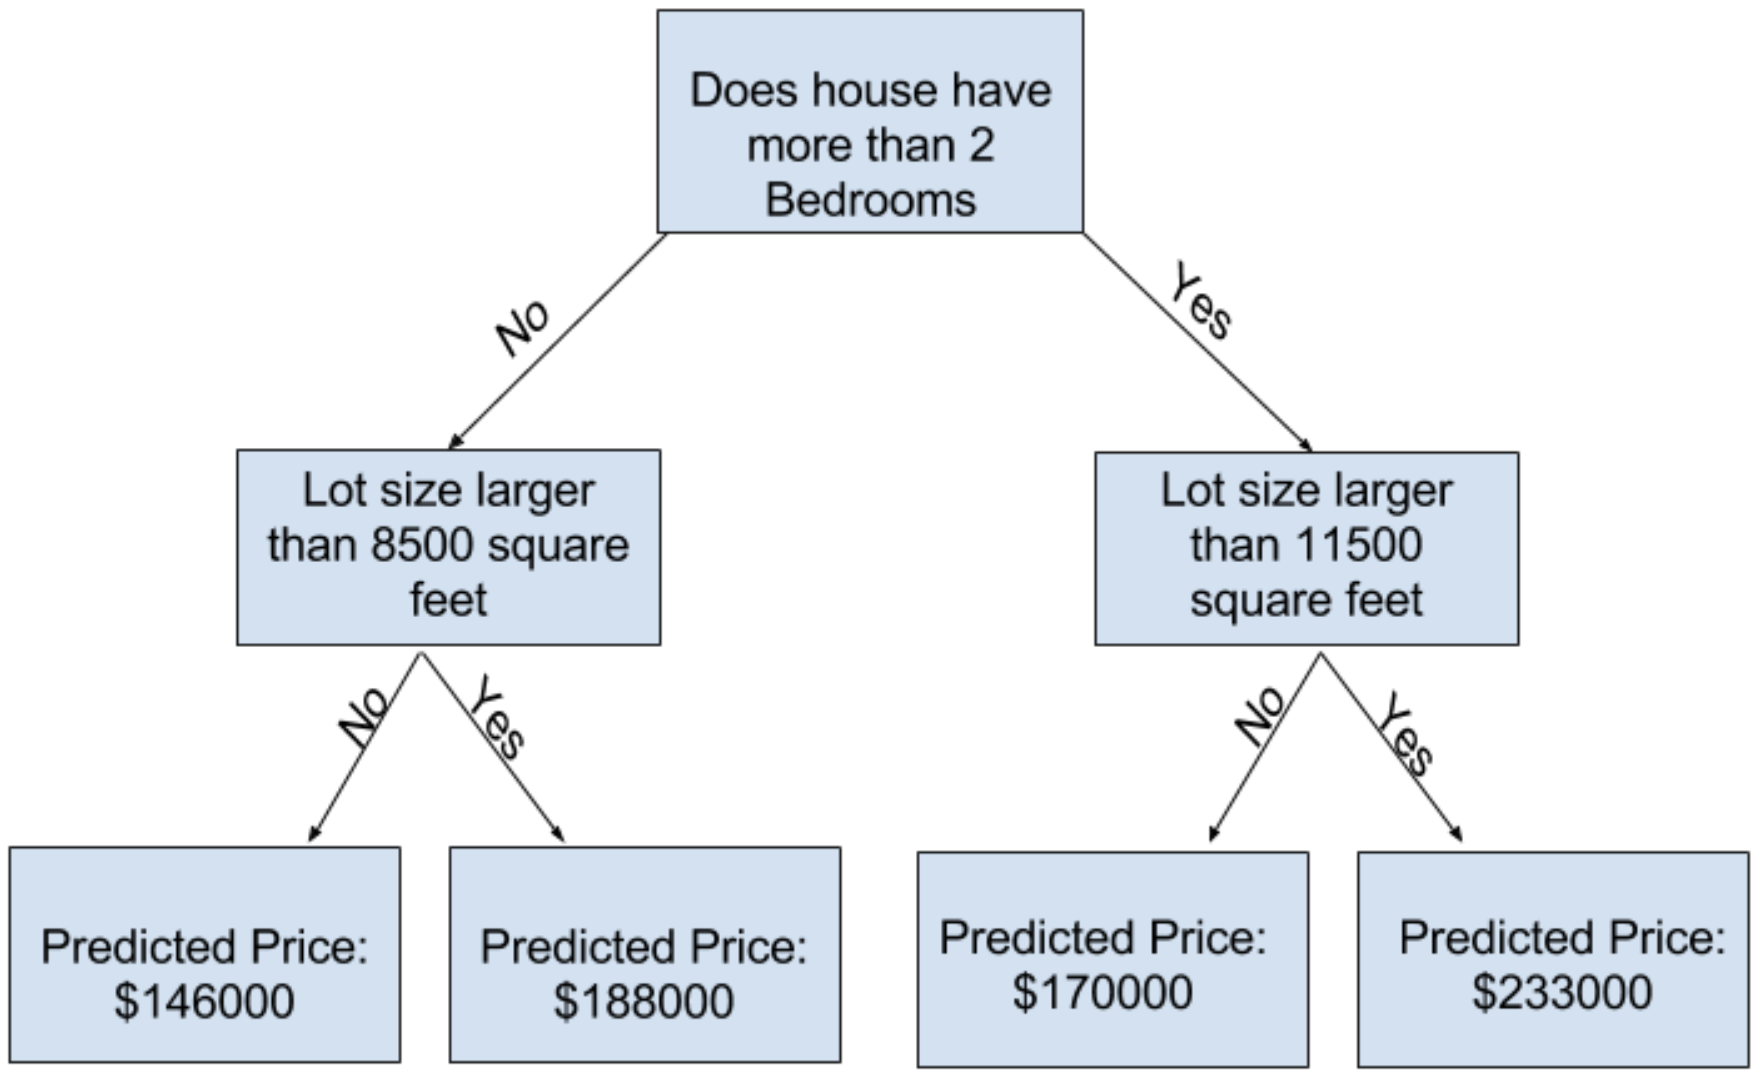
\includegraphics[scale=0.5]{image2.png}

    Deeper Trees
\end{figure}

    \chapter{Перевірка моделі}\label{cha:model_validation}
Майже кожну, яку ми не створювали модель, треба оцінювати на наявність помилок.
У більшості (хоча і не у всіх) застосуваннях відповідним показником якості моделі є точність прогнозування.
Іншими словами, чи будуть \textit{прогнози моделі близькими до того, що насправді відбувається}.

Існує багато метрик для підведення підсумків якості моделі, але в даній роботі буде застосована середня абсолютна помилка (також звана MAE).

Помилка передбачення суми для кожного будинку:
\[error=actual-predicted\]
Отже, якщо будинок коштував \$150 000, і ви передбачали, що він коштуватиме \$100 000, помилка становить \$50 000.
За допомогою метрики MAE ми приймаємо \textit{абсолютне значення} кожної помилки.
Це перетворює кожну помилку на додатне число.
Потім беремо середнє значення цих абсолютних помилок.
Це наш показник якості моделі.
Інакше кажучи, у середньому наші прогнози відхиляються приблизно на X.

Для розрахунку MAE нам спочатку потрібна модель.

\begin{lstlisting}[style=light, language=Python,label={lst:vectorimg},caption=Розрахунок середньої абсолютної похибки]
        from sklearn.metrics import mean_absolute_error

        predicted_home_prices = melbourne_model.predict(X)
        print(mean_absolute_error(y, predicted_home_prices))
        # 434.71594577146544
\end{lstlisting}

\section{Проблема з оцінками <<в вибірці>>}\label{sec:in_sample_problem}
Значення, яки ми щойно обчислили, можна назвати оцінкою "у вибірці".
Ми використовували єдиний "зразок" будинків як для побудови моделі, так і для її оцінки.

Модель буде вважатися точною у даних тренінгу.
Модель буде дуже неточною при використанні на практиці, оскільки натренована модель не буде розпізновати нові дані, тому як шаблон не виконується.

Практична цінність моделей полягає в прогнозуванні нових даних, ми вимірюємо ефективність даних, які не використовувались для побудови моделі.
Найпростіший спосіб зробити це - виключити деякі дані з процесу побудови моделі, а потім використовувати їх для перевірки точності моделі на даних, яких вона раніше не бачила.
Ці дані називаються \textbf{даними перевірки}.

\begin{lstlisting}[style=light, language=Python,label={lst:vectorimg},caption=The mean absolute error calculcation]
        from sklearn.model_selection import train_test_split

        # split data into training and validation data, for both features and target
        # The split is based on a random number generator. Supplying a numeric value to
        # the random_state argument guarantees we get the same split every time we
        # run this script.
        train_X, val_X, train_y, val_y = train_test_split(X, y, random_state = 0)
        # Define model
        melbourne_model = DecisionTreeRegressor()
        # Fit model
        melbourne_model.fit(train_X, train_y)

        # get predicted prices on validation data
        val_predictions = melbourne_model.predict(val_X)
        print(mean_absolute_error(val_y, val_predictions))
        # 263007.8766946417
\end{lstlisting}

\section{Переобладнанням та недооснащенням}\label{sec:underfitting_overfitting}
На практиці нерідкі випадки, коли дерево має 10 розщеплень між верхнім рівнем (усі будинки) та листом.
По мірі того, як дерево стає глибшим, набір даних нарізається на листя з меншою кількістю будинків.
Якщо дерево мало лише 1 поділ, воно ділить дані на 2 групи.
Якщо кожну групу розділити знову, ми отримаємо 4 групи будинків.
Поділ кожного з них знову створить 8 груп.
Якщо ми продовжуватимемо подвоювати кількість груп, додаючи більше розділень на кожному рівні, до того, як дійдемо до 10-го рівня, у нас буде \ (2 ^ 10 \) груп будинків.
Це 1024 листки.

Коли ми ділимо будинки на багато листків, у нас також менше будинків в кожному листку.
Листя з дуже малою кількістю будинків даватимуть прогнози, які досить близькі до фактичних значень цих будинків, але вони можуть робити дуже ненадійні прогнози щодо нових даних (оскільки кожен прогноз базується лише на кількох будинках).

Це явище, яке називається \textbf{перенавчання(overfitting)}, коли модель майже ідеально відповідає навчальним даним, але погано справляється з валідацією та іншими новими даними.
З іншого боку, якщо ми зробимо наше дерево дуже дрібним, воно не ділить будинки на унікальні групи.

У крайньому випадку, якщо дерево ділить будинки лише на 2 або 4, кожна група все ще зберігає властивість різноманітності.
Очікувані прогнози можуть бути не точними для більшості будинків, навіть у даних для тренування (і це також буде погано у валідації з тієї ж причини).
Коли модель не може вловити важливі відмінності та закономірності в даних, вона буде погано працювати з навчальними даними, що називається \textbf{переобладнаннямм (underfitting)}.

Оскільки ми дбаємо про точність нових даних, які ми оцінюємо на основі наших даних перевірки, ми хочемо знайти найкращу точку між переобладнанням та недооснащенням.
Візуально нам потрібна нижня точка (червоної) кривої перевірки (див. Малюнок 3).

\begin{figure}
    \label{fig:image3}
    \centering
    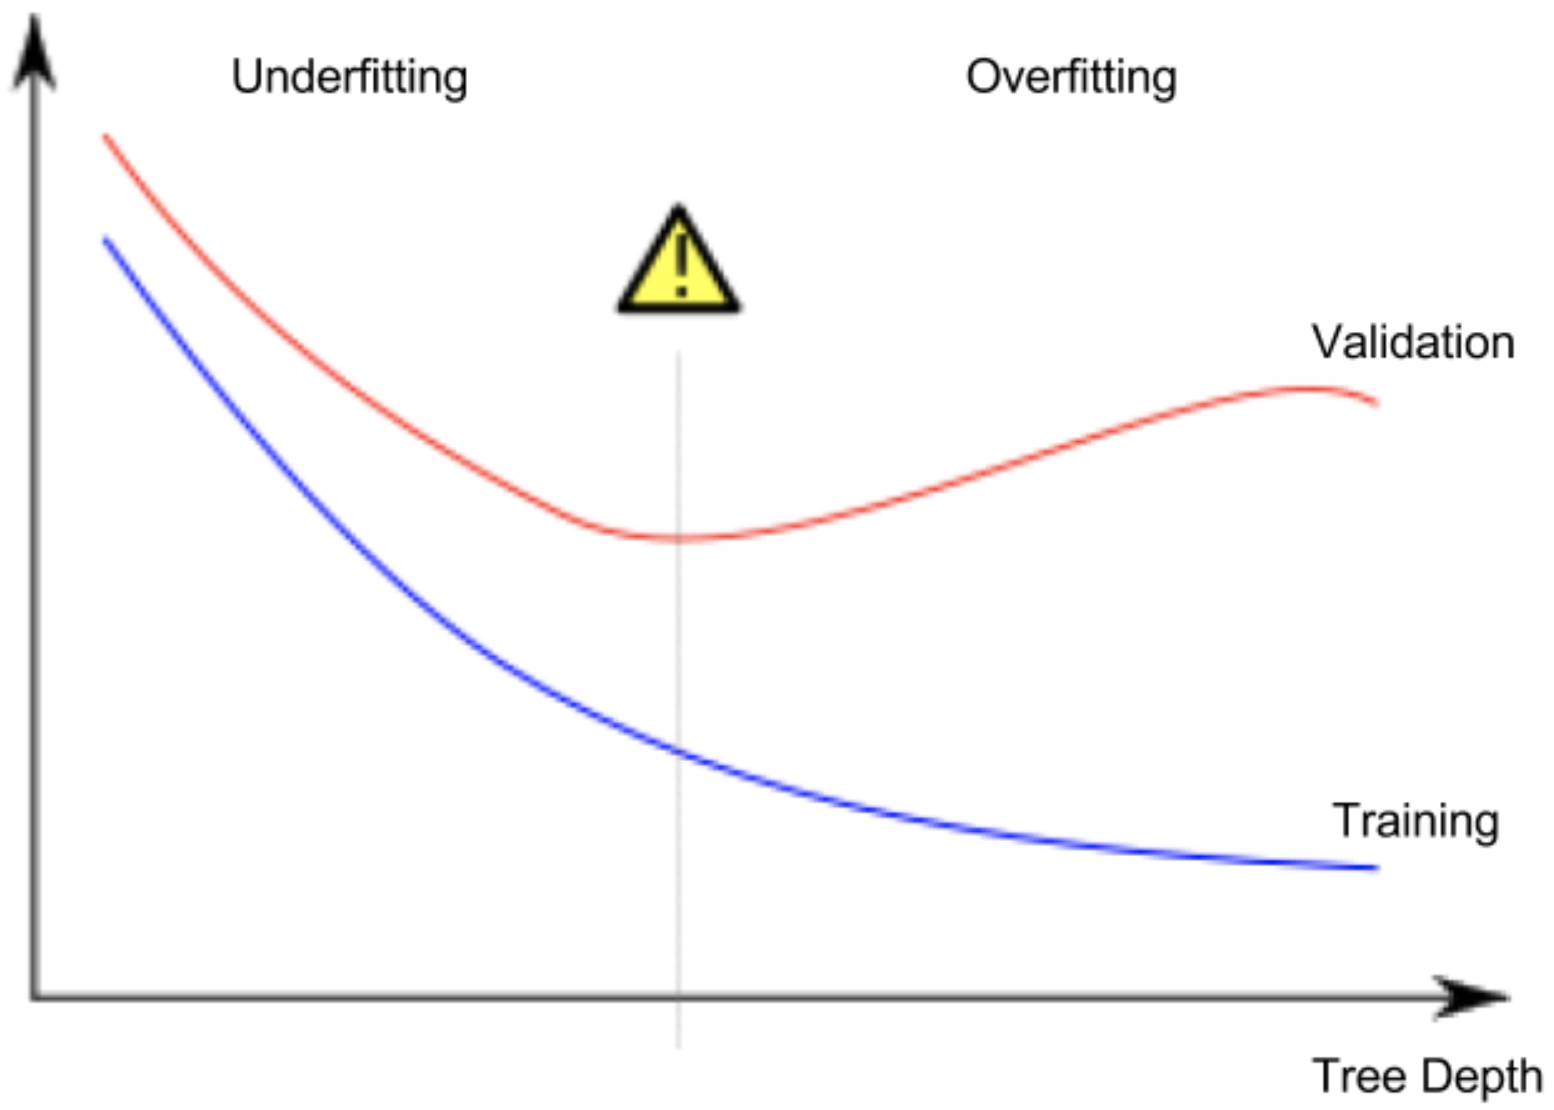
\includegraphics[scale=0.5]{image3.png}

    Deeper Trees
\end{figure}

    \chapter{Оптимізація моделі. Вибираємо оптимальне значення рівнів дерева}\label{cha:selecting_number_of_leafs}
Існує кілька альтернатив для управління глибиною дерева, і багато з них дозволяють, щоб деякі маршрути через дерево мали більшу глибину, ніж інші маршрути.
Але аргумент \textbf{max\_leaf\_nodes} забезпечує спосіб контролювати переобладнанням та недооснащенням облаштування.
Чим більше аркушів ми дозволяємо зробити моделі, тим більше ми переходимо від зони недообладнання на наведеному графіку до зони переоснащення.

Ми можемо використовувати функцію корисності, щоб допомогти порівняти оцінки MAE з різних значень для \textbf{max\_leaf\_nodes}.

З перелічених варіантів 500 - це оптимальна значення для нашої моделі.

\begin{lstlisting}[style=light, language=Python,label={lst:vectorimg},caption=Computing MAE for different value of leaf nodes]
from sklearn.metrics import mean_absolute_error
from sklearn.tree import DecisionTreeRegressor

def get_mae(max_leaf_nodes, train_X, val_X, train_y, val_y):
    model = DecisionTreeRegressor(max_leaf_nodes=max_leaf_nodes, random_state=0)
    model.fit(train_X, train_y)
    preds_val = model.predict(val_X)
    mae = mean_absolute_error(val_y, preds_val)
    return(mae)

# compare MAE with differing values of max_leaf_nodes
for max_leaf_nodes in [5, 50, 500, 5000]:
    my_mae = get_mae(max_leaf_nodes, train_X, val_X, train_y, val_y)
    print("Max leaf nodes: %d  \t\t Mean Absolute Error:  %d" %(max_leaf_nodes, my_mae))

# Max leaf nodes: 5  		 Mean Absolute Error:  347380
# Max leaf nodes: 50  		 Mean Absolute Error:  258171
# Max leaf nodes: 500  		 Mean Absolute Error:  243495
# Max leaf nodes: 5000       Mean Absolute Error:  254983
\end{lstlisting}

    \chapter{Випадковий ліс дерев}\label{cha:random_forest_tree}
Дерева рішень залишають за вами важке рішення.
Глибоке дерево з великою кількістю рівнів перевантажиться, тому що кожне передбачення походить із історичних даних лише кількох будинків на його листі.
Але неглибоке дерево з невеликою кількістю листя буде працювати погано, оскільки воно не вловлює стільки відмінностей у вихідних даних.

Навіть найскладніші техніки моделювання сьогодні стикаються з проблемою між недооснащенням та переобладнанням.

У випадковому лісі використовується багато дерев, і він робить прогноз, усереднюючи прогнози кожного дерева компонентів.
Як правило, він має набагато кращу точність прогнозування, ніж одне дерево рішень, ця модель добре працює з параметрами за замовчуванням.

Випадковий ліс дерев демонструє значне ліпші результати порівняно з попереднім рішенням з одним деревом та помилкою у 250 000.

\begin{lstlisting}[style=light, language=Python,label={lst:vectorimg},caption=Random Forest Tree]
        from sklearn.ensemble import RandomForestRegressor
        from sklearn.metrics import mean_absolute_error

        forest_model = RandomForestRegressor(random_state=1)
        forest_model.fit(train_X, train_y)
        melb_preds = forest_model.predict(val_X)
        print(mean_absolute_error(val_y, melb_preds))
        # 191669.7536453626
\end{lstlisting}


    \backmatter %% Здесь заканчивается нумерованная часть документа и начинаются ссылки и
    %% заключение

    \Conclusion % заключение к отчёту

Моделі можуть страждати від:

\begin{itemize}
    \item \textbf{Переобладнанням}: захоплення помилкових патернів, які не повторяться в майбутньому, що призведе до менш точних прогнозів, або
    \item \textbf{Недооснащенням}: не вдалося вловити відповідні закономірності, що знову призводить до менш точних прогнозів.
\end{itemize}
Ми використовуємо дані перевірки, які не використовуються при навчанні моделей, для вимірювання точності кандидатської моделі.
Це дозволяє нам спробувати багато моделей кандидатів і зберегти найкращу.

Є параметри, які дозволяють вам нам ефективність випадкового лісу настільки, наскільки ми змінили максимальну глибину одного дерева рішень.
Але однією з найкращих особливостей моделей Random Forest є те, що вони, як правило, прогнозують дуже добро навіть без додаткової настройки.


    \nocite{*}
\bibliographystyle{gost780u}
\bibliography{0-main}


\end{document}
